% !TeX root = ../dokumentation.tex

\chapter{Teamorganisation}

\section{Rollenverteilung}
    Zusätzlich zu den klassischen Scrum-Rollen Product-Owner, Scrum-Master und Entwickler 
    wurden im Projekt weitere Rollen eingeführt: Architekten und Service-Leads (vgl. \ref*{fig:Rollenverteilung}). 
    Grundsätzliches Ziel war es die Komplexität des Projektes durch Arbeitsteiltung und feste Ansprechpartner abzufangen.
    Damit sollte auch eine Zusammenarbeit trotz verschiedener Kenntnisstände zu ermöglichen und einen Wissensaustausch zu erleichtern.   

    Die Aufgabe des Produkt-Owners ist es, den Wert des Produkts bzw. des Projekts
    zu maximieren. Mit Hilfe des Backlogs und der Priorisierung der Aufgaben darin stellt der Produkt Owner
    sicher, dass das Team an den richtigen Aufgaben arbeitet.
    Zusätzlich wurden in unserem Team die Storys vom Product Owner erstellt und die Estimation- sowie Planning-Meetings geplant.

    Ein Scrum-Master ist vergleichbar mit einem Teamleiter. Er kümmert sich darum, dass
    das Team (Entwickler und PO) ihrer Arbeit bestmöglich nachgehen können und schützt
    das Team vor ungewolltem Einfluss von außen. Zusammenfassend kann
    man sagen, dass der Scrum-Master dafür verantwortlich ist, dass sich das Team selbst
    organisieren und arbeiten kann. Der Scrum-Master hat auch die Aufgabe, darauf zu achten, dass das Team sich an die
    Scrum-Regeln hält, also alle Meetings regelmäßig durchgeführt werden und tritt wenn nötig in den Meetings als Moderator auf.

    Die Architekten sind für die grundsätzliche Infrastruktur im Projekt zuständig. 
    Dazu entwarfen sie eine Service-übergreifende Architektur und bestimmten nach Evalurierung die eingesetzten Technologien.
    Ziel war es, dass die Architekten einen Gesamtüberblick über das Projekt behalten, 
    und somit Kommunikation zwischen den Services ermöglichen.
     
    
    Service-Leads sind die Ansprechpartner für die einzelnen Services. Dabei sollen sie einen detaillierteren Überblick über die Services behalten 
    und bei Fragen des Teams zur Verfügung stehen. 
    Da die Service-Leads einen besseren Überblick über den Service haben, 
    übernehmen sie by default die Review von service-spezifischen Tickets und Pull-Requests in den Service-Repositories.

    \begin{figure}
        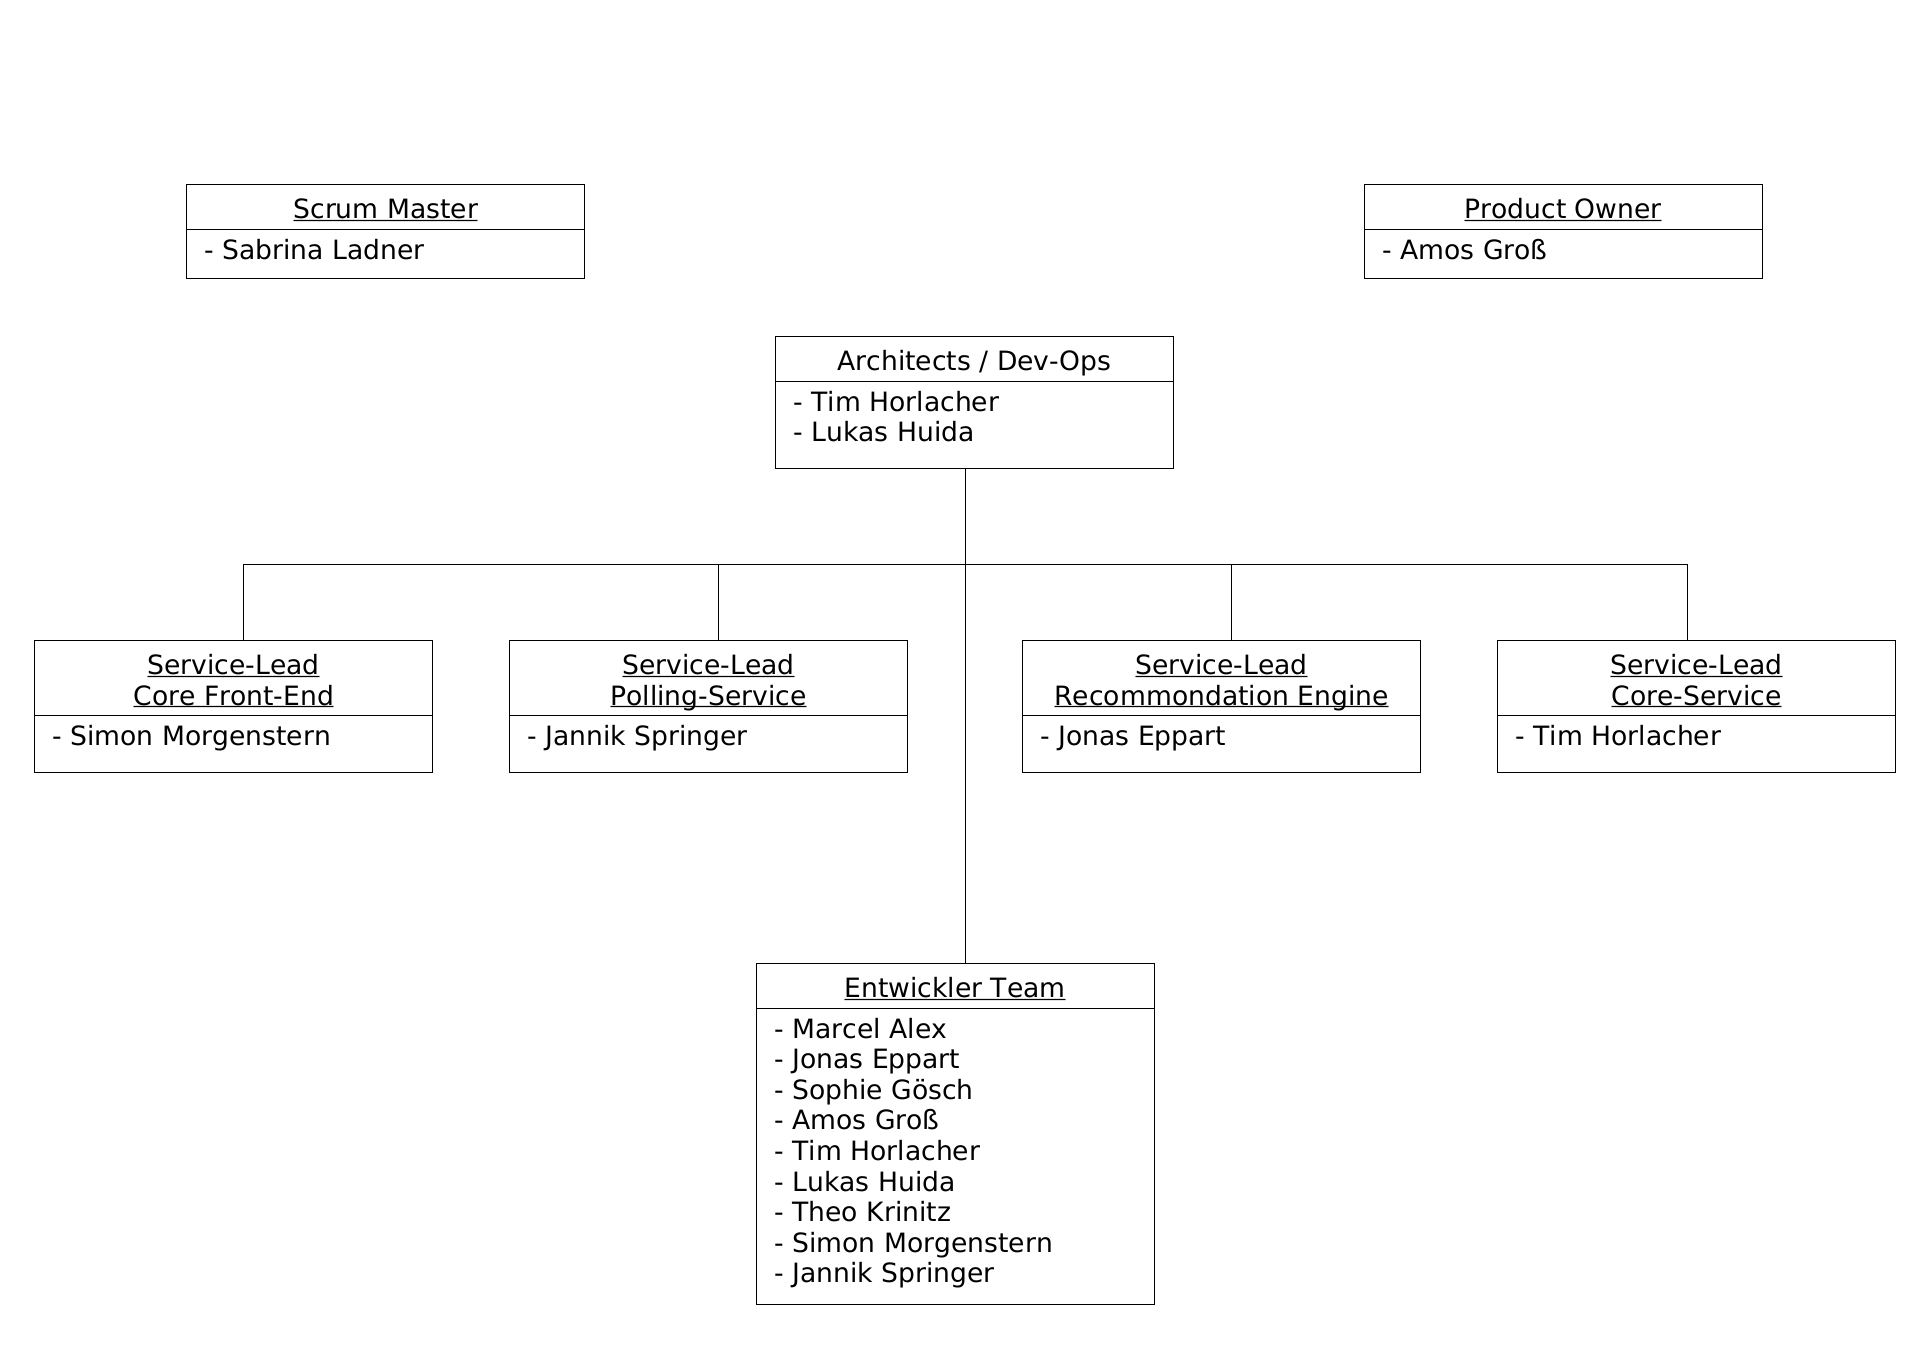
\includegraphics[width=\linewidth]{ProjektOrganigramm2.png}
        \caption{Rollenverteilung}
        \label{fig:Rollenverteilung}
    \end{figure}
    
\section{Eingesetzte Technologien}

\section{Zusammenarbeit}
\todo{Meetings und co}